\documentclass{thesisby}

%%%кодировка...
\usepackage[utf8]{inputenc}
\usepackage[T1,T2A]{fontenc}

\usepackage[english, russian]{babel}

%%%для борьбы с переполнениями за счет разреженных слов в абзаце
\emergencystretch=25pt

\usepackage{amsmath,amssymb,amsfonts}

\usepackage{longtable,array, multirow}

\usepackage{graphicx,epsfig}

%%%для чернового режима работы%%%
%%%раскоментить при создании электронной версии с гиперссылками
%\usepackage[unicode,colorlinks,pagebackref]{hyperref}
%\usepackage[unicode]{hyperref}
%\usepackage{refcheck}% checks lost and useless labels, shows `keys' of \label in the margins
%%%для времени сборки на титульном черновика
\usepackage{datetime}
%%%чтобы зачеркивать слова
\usepackage{ulem}
% в тексте, чтобы вычеркнуть слово
%\sout{Неправильно.} Правильно.

%%%конец___для чернового режима работы%%%

\usepackage{textcomp}% For Celsium sign only \textcelsius

%%%картинки eps тут:
\graphicspath{{fig/}}

%%%интервал строк
\usepackage{setspace}
% одинарный интервал
\singlespacing
% полуторный интервал
%\onehalfspacing
% двойной интервал
%\doublespacing
% произвольный интервал
%\setstretch{line_spacing_value}
%Для блока с текстом, например, можно сжать часть текста по вертикали
%\begin{singlespacing}
%...
%\end{singlespacing}
%или
%\begin{spacing}{1.0}
%...
%\end{spacing}





%%%как сделать в латехе чтобы он писал [1-10]? 
%\usepackage{cite}  % \cite{Petrov, Sidorov...}


%%% will be using font like `Times New Roman'
\usepackage{pscyr}
\renewcommand{\rmdefault}{ftm}

%%%current file is THESIS?
%%%YES - isthesis=1
%%%NO - isthesis=0
\usepackage{ifthen}
\newcounter{isthesis}
\setcounter{isthesis}{1}

%%%для подсчета общего количества страниц в общую характеристику
%\usepackage{lastpage}



\title{thesis}
\author{Vincent Vega}
\date{\currenttime}




%%%для поворота страницы альбомом
\usepackage{lscape}


%%%заполнения точками всех уровней содержания/огравления
\makeatletter
\renewcommand*\l@chapter{\hskip 0pt \@dottedtocline{1}{0.0em}{0em}}
%\renewcommand*\l@chapter{\hskip 0pt \vspace{10pt} \@dottedtocline{1}{0.0em}{2.3em}}
%\renewcommand*\l@section{\@dottedtocline{1}{1.5em}{2.3em}}
%\renewcommand*\l@chapter{\@dottedtocline{1}{1.5em}{2.3em}}
%\renewcommand*\l@chapter{\hskip 0pt \vspace{-20pt} \@dottedtocline{1}{1.5em}{2.3em}}
%\renewcommand*\l@chapter{\hskip -50pt \hspace{-120pt} \@dottedtocline{1}{1.5em}{2.3em}}
\makeatother


%%%убрать переносы в словах:
\hyphenation{НИИСФ БНТУ МГСУ НИПТИС РААСН БелНИИС}

%%%для дополнительных символов/используется в подписям к рис гл1
%\usepackage{fdsymbol}
\usepackage{MnSymbol}
%\usepackage{mathabx}

%%%для отключения переноса section в приложениях в содержание
%http://mydebianblog.blogspot.com/2011/05/latex.html
%Уровень подробности останется тем же до следующей команды \settocdepth. Например, в Appendix я не хочу отображать подразделы вовсе:   \settocdepth{chapter}
\usepackage{tocvsec2}


%%%последовательно переносы в строках до 1000000. default 10000
%\doublehyphendemerits=10000
%Замечу, что пробел между словами "резиновое расстояние" (растягивается и сжимается). Пакет microtype помогает оптимизации. Просто загрузите -- и все
\usepackage{microtype}


%%%для греческий букв прямого начертания
%%https://dxdy.ru/post985777.html#p985777

%% Определяем свой шрифт "greek"
\DeclareSymbolFont{greek}{U}{eur}{m}{n}
\SetSymbolFont{greek}{bold}{U}{eur}{b}{n}
\DeclareSymbolFontAlphabet{\gr}{greek}

%% Определяем буквы
\DeclareMathSymbol{\alpha}{\mathord}{greek}{"0B}
\DeclareMathSymbol{\beta}{\mathord}{greek}{"0C}
\DeclareMathSymbol{\gamma}{\mathord}{greek}{"0D}
\DeclareMathSymbol{\delta}{\mathord}{greek}{"0E}
\DeclareMathSymbol{\epsilon}{\mathord}{greek}{"0F}
\DeclareMathSymbol{\zeta}{\mathord}{greek}{"10}
\DeclareMathSymbol{\eta}{\mathord}{greek}{"11}
\DeclareMathSymbol{\theta}{\mathord}{greek}{"12}
\DeclareMathSymbol{\iota}{\mathord}{greek}{"13}
\DeclareMathSymbol{\kappa}{\mathord}{greek}{"14}
\DeclareMathSymbol{\lambda}{\mathord}{greek}{"15}
\DeclareMathSymbol{\mu}{\mathord}{greek}{"16}
\DeclareMathSymbol{\nu}{\mathord}{greek}{"17}
\DeclareMathSymbol{\xi}{\mathord}{greek}{"18}
\DeclareMathSymbol{\pi}{\mathord}{greek}{"19}
\DeclareMathSymbol{\rho}{\mathord}{greek}{"1A}
\DeclareMathSymbol{\sigma}{\mathord}{greek}{"1B}
\DeclareMathSymbol{\tau}{\mathord}{greek}{"1C}
\DeclareMathSymbol{\upsilon}{\mathord}{greek}{"1D}
\DeclareMathSymbol{\phi}{\mathord}{greek}{"1E}
\DeclareMathSymbol{\chi}{\mathord}{greek}{"1F}
\DeclareMathSymbol{\psi}{\mathord}{greek}{"20}
\DeclareMathSymbol{\omega}{\mathord}{greek}{"21}
\DeclareMathSymbol{\varepsilon}{\mathord}{greek}{"22}
\DeclareMathSymbol{\vartheta}{\mathord}{greek}{"23}
\DeclareMathSymbol{\varpi}{\mathord}{greek}{"24}
%% В AMS-овском шрифте  \varrho и \varsigma нет
\let\varrho\rho
\let\varsigma\sigma
\DeclareMathSymbol{\varphi}{\mathord}{greek}{"27}
%%https://dxdy.ru/post986322.html#p986322

%%%%%%%%%%%%%%%%%%%%%%%%%%%%%%%%%%%%%%%%%%%%%%%%%%%%%%%%%%%%%%%%%%%%%%%%%%
%%%                                                                    %%%
%%%              Вставить эти макрокоманды в преамбулу                 %%%
%%%                                                                    %%%
%%%%%%%%%%%%%%%%%%%%%%%%%%%%%%%%%%%%%%%%%%%%%%%%%%%%%%%%%%%%%%%%%%%%%%%%%%
%%%%%%%%%%%%%%%%%%%%%%%%%%%%%%%%%%%%%%%%%%%%%%%%%%%%%%%%%%%%%%%%%%%%%%%%%%
%                                                                      %%%
%%%  Задаем новый шрифт (для автоматического масштабирования индексов) %%%
%                                                                      %%%
\DeclareFontFamily{OT1}{mygreek}{}%                                    %%%
\DeclareFontShape{OT1}{mygreek}{m}{n}{<->omsegr}{}%                    %%%
\DeclareSymbolFont{Greekrm}{OT1}{mygreek}{m}{n}                        %%%
%                                                                      %%%
%%%  Переопределяем греческие буквы, в т.ч. большие (например, \Omega  %%%
%%%  в оригинале плохая, остальные переопределяем для единства стиля)  %%%
%                                                                      %%%
\DeclareMathSymbol{\Alpha}{\mathalpha}{Greekrm}{65}                    %%%
\DeclareMathSymbol{\Beta}{\mathalpha}{Greekrm}{66}                     %%%
\DeclareMathSymbol{\Gamma}{\mathalpha}{Greekrm}{71}                    %%%
\DeclareMathSymbol{\Delta}{\mathalpha}{Greekrm}{68}                    %%%
\DeclareMathSymbol{\Epsilon}{\mathalpha}{Greekrm}{69}                  %%%
\DeclareMathSymbol{\Zeta}{\mathalpha}{Greekrm}{90}                     %%%
\DeclareMathSymbol{\Eta}{\mathalpha}{Greekrm}{72}                      %%%
\DeclareMathSymbol{\Theta}{\mathalpha}{Greekrm}{74}                    %%%
\DeclareMathSymbol{\Iota}{\mathalpha}{Greekrm}{73}                     %%%
\DeclareMathSymbol{\Kappa}{\mathalpha}{Greekrm}{75}                    %%%
\DeclareMathSymbol{\Lambda}{\mathalpha}{Greekrm}{76}                   %%%
\DeclareMathSymbol{\Mu}{\mathalpha}{Greekrm}{77}                       %%%
\DeclareMathSymbol{\Nu}{\mathalpha}{Greekrm}{78}                       %%%
\DeclareMathSymbol{\Omicron}{\mathalpha}{Greekrm}{79}                  %%%
\DeclareMathSymbol{\Xi}{\mathalpha}{Greekrm}{88}                       %%%
\DeclareMathSymbol{\Pi}{\mathalpha}{Greekrm}{80}                       %%%
\DeclareMathSymbol{\Rho}{\mathalpha}{Greekrm}{82}                      %%%
\DeclareMathSymbol{\Sigma}{\mathalpha}{Greekrm}{83}                    %%%
\DeclareMathSymbol{\Tau}{\mathalpha}{Greekrm}{84}                      %%%
\DeclareMathSymbol{\Upsilon}{\mathalpha}{Greekrm}{85}                  %%%
\DeclareMathSymbol{\Phi}{\mathalpha}{Greekrm}{70}                      %%%
\DeclareMathSymbol{\Chi}{\mathalpha}{Greekrm}{81}                      %%%
\DeclareMathSymbol{\Psi}{\mathalpha}{Greekrm}{89}                      %%%
\DeclareMathSymbol{\Omega}{\mathalpha}{Greekrm}{87}                    %%%
%                                                                      %%%
\DeclareMathSymbol{\alpha}{\mathalpha}{Greekrm}{97}                    %%%
\DeclareMathSymbol{\beta}{\mathalpha}{Greekrm}{98}                     %%%
\DeclareMathSymbol{\varbeta}{\mathalpha}{Greekrm}{49}                  %%%
\DeclareMathSymbol{\gamma}{\mathalpha}{Greekrm}{103}                   %%%
\DeclareMathSymbol{\delta}{\mathalpha}{Greekrm}{100}                   %%%
\DeclareMathSymbol{\epsilon}{\mathalpha}{Greekrm}{101}                 %%%
\DeclareMathSymbol{\varepsilon}{\mathalpha}{Greekrm}{101}              %%%
\DeclareMathSymbol{\zeta}{\mathalpha}{Greekrm}{122}                    %%%
\DeclareMathSymbol{\eta}{\mathalpha}{Greekrm}{104}                     %%%
\DeclareMathSymbol{\theta}{\mathalpha}{Greekrm}{106}                   %%%
\DeclareMathSymbol{\vartheta}{\mathalpha}{Greekrm}{50}                 %%%
\DeclareMathSymbol{\iota}{\mathalpha}{Greekrm}{105}                    %%%
\DeclareMathSymbol{\kappa}{\mathalpha}{Greekrm}{107}                   %%%
\DeclareMathSymbol{\varkappa}{\mathalpha}{Greekrm}{53}                 %%%
\DeclareMathSymbol{\lambda}{\mathalpha}{Greekrm}{108}                  %%%
\DeclareMathSymbol{\mu}{\mathalpha}{Greekrm}{109}                      %%%
\DeclareMathSymbol{\nu}{\mathalpha}{Greekrm}{110}                      %%%
\DeclareMathSymbol{\omicron}{\mathalpha}{Greekrm}{111}                 %%%
\DeclareMathSymbol{\xi}{\mathalpha}{Greekrm}{120}                      %%%
\DeclareMathSymbol{\pi}{\mathalpha}{Greekrm}{112}                      %%%
\DeclareMathSymbol{\varpi}{\mathalpha}{Greekrm}{55}                    %%%
\DeclareMathSymbol{\rho}{\mathalpha}{Greekrm}{114}                     %%%
\DeclareMathSymbol{\varrho}{\mathalpha}{Greekrm}{52}                   %%%
\DeclareMathSymbol{\sigma}{\mathalpha}{Greekrm}{115}                   %%%
\DeclareMathSymbol{\varsigma}{\mathalpha}{Greekrm}{99}                 %%%
\DeclareMathSymbol{\tau}{\mathalpha}{Greekrm}{116}                     %%%
\DeclareMathSymbol{\upsilon}{\mathalpha}{Greekrm}{117}                 %%%
\DeclareMathSymbol{\phi}{\mathalpha}{Greekrm}{102}                     %%%
\DeclareMathSymbol{\varphi}{\mathalpha}{Greekrm}{51}                   %%%
\DeclareMathSymbol{\chi}{\mathalpha}{Greekrm}{113}                     %%%
\DeclareMathSymbol{\psi}{\mathalpha}{Greekrm}{121}                     %%%
\DeclareMathSymbol{\omega}{\mathalpha}{Greekrm}{119}                   %%%
%                                                                      %%%
%%%%%%%%%%%%%%%%%%%%%%%%%%%%%%%%%%%%%%%%%%%%%%%%%%%%%%%%%%%%%%%%%%%%%%%%%%
%%%%%%%%%%%%%%%%%%%%%%%%%%%%%%%%%%%%%%%%%%%%%%%%%%%%%%%%%%%%%%%%%%%%%%%%%%




\begin{document}



%%%раскоментить при создании электронной версии с гиперссылками
%это отображается в свойствах файла pdf при включенном {hyperref} (см в этом файле выше)
%\hypersetup{
%pdftitle = {Изучение возможностей использования каши в голове в качестве пищи для ума},
%pdfauthor = {Вега Винсент Траволтович},
%pdfsubject = {Диссертация на соискание ученой степени кандидата технических наук},
%pdfkeywords = {фильм, винсент, тарантино, уоллес, роль, сцена, джулс, бутч, мия, сценарий}
%}% End of hypersetup






%ТИТУЛЬНЫЙ ЛИСТ
\begin{titlepage}

\begin{center} \bfseries
 Национальная академия наук Беларуси \\
\bigskip
{ГОСУДАРСТВЕННОЕ НАУЧНОЕ УЧРЕЖДЕНИЕ}
\medskip

{<<ОБЪЕДИНЕННЫЙ ИНСТИТУТ ЭНЕРГЕТИЧЕСКИХ
И ЯДЕРНЫХ ИССЛЕДОВАНИЙ – СОСНЫ>>}
\end{center}
\medskip

\noindent На правах рукописи\\
УДК  123.456 \\
\vspace{1cm}

\begin{center}
{\large ПЕТРОВ \\ Вадим Александрович}\\ \vspace{1cm}

{\bfseries Руководство по оформлению диссертации с использованием \TeX овского класса {\itshape thesisby} версии 1.1}\\
\vspace{2cm}
Диссертация на соискание ученой степени\\
кандидата физ. - \TeX{} наук\\
\medskip

по специальности 12.34.56 \TeX ника
\end{center}
\vspace{3cm}

\begin{tabbing}
\hspace{8cm} \= \kill \>
Научный руководитель \+ \\
д-р физ. - \TeX{} наук, профессор\\
Петров А.В.
\end{tabbing}
\vspace{5cm}

\begin{center}
 \bfseries Минск 2016
\end{center}

\end{titlepage}



%ОГЛАВЛЕНИЕ
\tableofcontents

%ПЕРЕЧЕНЬ УСЛОВНЫХ ОБОЗНАЧЕНИЙ
\newpage
\chapter*{ПЕРЕЧЕНЬ УСЛОВНЫХ ОБОЗНАЧЕНИЙ}
\addcontentsline{toc}{chapter}{ПЕРЕЧЕНЬ УСЛОВНЫХ ОБОЗНАЧЕНИЙ}

\noindent %подавление абзацаного отступа
$c_{T}$ -- удельная теплоёмкость, Дж/(кг$\cdot^\circ$C);\\
$t$ -- температура, $^\circ$C;\\
$t_\text{в}$ -- температура внутреннего воздуха, $^\circ$C;\\
$\Delta t$ -- перепад температуры, $^\circ$C;\\
$\lambda_{T}$  -- коэффициент теплопроводности, Вт/(м$\cdot^\circ$C);\\
$\tau$ -- время, с;\\
$\varphi$ -- относительная влажность воздуха, в долях единицы или \%.\\



Остальные обозначения приведены согласно первоисточникам и дополнительно расшифрованы.



%ВВЕДЕНИЕ


\newpage
\chapter*{ВВЕДЕНИЕ}
\addcontentsline{toc}{chapter}{ВВЕДЕНИЕ}

%Проблема1
Некий текст.


%Проблема2
Некий текст.



%Проблема5
%\pagebreak
Некий текст.


%Заключение
%\pagebreak
Анализируя сказанное выше,
приходим к выводу, что каша в голове находится у большинства индивидуумов.
Поэтому изучение возможностей использования её в качестве пищи для ума является основой экстенсивного развития нашего общества, экономики страны и мира. 
В связи с этим результаты исследований, представленные в настоящей работе, являются весьма востребованными.





%ОБЩАЯ ХАРАКТЕРИСТИКА РАБОТЫ

%\newpage
\chapter*{ОБЩАЯ ХАРАКТЕРИСТИКА РАБОТЫ} ~
\addcontentsline{toc}{chapter}{ОБЩАЯ ХАРАКТЕРИСТИКА РАБОТЫ}~

\vspace{-16pt}
%\subsubsection*{Связь работы с научными программами (проектами), темами.}
\textbf{Связь работы с научными программами (проектами), темами}

Тема работы соответствует программе <<Переливание из пустого в порожнее>> приоритетных направлений научно-технической деятельности в Республике Беларусь на \mbox{2016--2020}~годы, утвержденных Указом Президента Республики Беларусь  \textnumero ~100500 от~30.02.2055.


\textbf{Цель и задачи исследования}

\textit{Цель работы}
-- откорректировать переработанный шаблон диссертации и залить в нет для его возможности использования другими поколениями ну и просто <<каб не прапала>>.

\textit{Объект исследований} -- абракадабра.

%\vspace{-20pt}
%\subsubsection*{Задачи исследований:}~
\textit{Задачи исследования:}

--~задачи исследования можно подгрузить из отдельного файла (прямо этого);

--~и его же можно подгрузить где-нибудь в литобзоре когда ставится задачи исследований;

--~хотя позже мне посоветовали текст задач изменить, чтобы не было дословного копирования из литобзора;

--~хотя, кому оно мешает в двух местах -- я так и не понял;

--~спишем на бюрократию.
%
%\ifthenelse{\value{isthesis}=0}{}{\pagebreak[4]}

%
%\vspace{-20pt}
%\subsubsection*{Научная новизна}работы:
%\pagebreak[4]
\textbf{Научная новизна} работы:

--~получены ...;

--~усовершенствована ...;

--~разработана ... .



%\vspace{-20pt}
%\subsubsection*{Положения, выносимые на защиту:}~
\ifthenelse{\value{isthesis}=0}{\pagebreak[4]}{}
\textbf{Положения, выносимые на защиту:}

--~результаты ...;

%\ifthenelse{\value{isthesis}=0}{\pagebreak[4]}{}

--~способ ...;

--~метод.


%\vspace{-20pt}
%\subsubsection*{Личный вклад соискателя.}~
\textbf{Личный вклад соискателя}~

Работа выполнена автором в Белорусском национальном техническом университете под руководством ...

Исследования ... проведены совместно с ...

Исследования ... выполнены совместно с ...

Остальные исследования ..., разработка математических моделей, ... и расчёты выполнены автором самостоятельно. 


%\vspace{-20pt}
%\subsubsection*{Апробация диссертации и информация об использовании ее результатов.}~
%\ifthenelse{\value{isthesis}=1}{\pagebreak[4]}{}
\textbf{Апробация диссертации и информация об использовании \linebreak ее результатов}~

Основные положения и результаты работы докладывались и обсуждались в рамках:

--~Научно-технических конференций <<ХХ>> \textnumero ~1--1 (2016--2019~гг.),  \textnumero ~1--5 (2002--2007~гг.);

--~V Международной практической конференции <<ХХ>>, Москва, 13 мая 2012~г.;

--~Научном семинаре <<ХХ>>, Санкт-Петербург, 23--24 июля 2001~г.;

--~Научно-практической конференции <<ХХ>>, Минск, 20 августа 2021~г.


%\vspace{-20pt}
%\subsubsection*{Опубликование результатов диссертации.}~
\textbf{Опубликование результатов диссертации}

По результатам работы опубликовано:

--\,пять статей в научных изданиях, соответствующих перечню ВАК Республики Беларусь;

--\,четыре статьи в научных изданиях, соответствующих перечню ВАК при Минобрнауки России;

--\,две статьи в научно-технических изданиях;

--\,пять публикаций в сборниках материалов и тезисов по результатам научно-технических конференций.


%\vspace{-20pt}
%\subsubsection*{Структура и объём диссертации.}~
\ifthenelse{\value{isthesis}=0}{\pagebreak[4]}{}
\textbf{Структура и объём диссертации}


Работа состоит из введения, общей характеристики работы, основной части, заключения,
списка использованных источников и приложений.

Основная часть работы состоит из 5 глав.

В первой главе выполнен ...

Вторая глава ...


В третьей главе ...


В главе 4 ...

\ifthenelse{\value{isthesis}=1}{\pagebreak[4]}{}
В главе 5...


Объём диссертации составляет ХХ страницы, в том числе основная часть YY страниц.
Основная часть содержит ZZ рисунков и TT таблиц.


%ОСНОВНАЯ ЧАСТЬ:
\chapter{ОБЗОРНАЯ}  \label{chapter1}


%%%надпись из [] идёт в содержание, надпись из {} идет заголовком в текст
\section[Очень очень длинное название первого параграфа]{Очень очень длинное название первого\\параграфа}\label{ch1-1}

Пример ссылки на литературу

@Article: \cite{PhysRevLett.116.167802, Polanyi1916, ermolenko1960}.

@Book: \cite{stallman2015free, trechsel2001}.

@Book: \cite{deriagin1984plenki, Lykov_stf}.

@Conference: \cite{capener2014art, art_krutilin_sorbcia2016}

@Electronic: \cite{bell2011pyamg, pogodaBY, vanovschi2015parallel}

@InCollection: \cite{Kuenzel_et_al_2001, bogoslovcky1966art}

@PhdThesis: \cite{descamps1996, kozlov_ktn}



@Manual (тут пишем всё что надо в поле Title): \cite{gost15588_2014}





\section[Еще один очень очень очень очень очень очень длинный заголовок]{Еще один очень очень очень очень очень очень\\длинный заголовок}\label{ch1-2}



Пример формулы:

\begin{equation}\label{eq:par_fokina}
\frac{\partial e}{\partial z} = \frac{\mu}{\xi_{o} \gamma}  E_{t} \frac{\partial^2 e}{\partial x^2},
\end{equation}

\begin{eqrem}
$x$ -- пространственная координата, м;\\
& $z$ -- временн\'{а}я координата, ч;\\
& $\mu$ -- коэффициент паропроницаемости материала, г/(м$\cdot$ч$\cdot$мм.рт.ст.);\\
& $\xi_{o}$ -- удельная относительная пароёмкость, г/кг;\\
& $\gamma$ -- объёмный вес материала, кг/м$^3$;\\
& $e$ -- упругость водяного пара, мм.рт.ст.;\\
& $E_{t}$ -- максимальная упругость водяного пара при температуре $t$, мм.рт.ст.
\end{eqrem}


Ещё один пример формулы:


\begin{equation}\label{eq:lukianov_t}
\begin{split}
\left( c_{o} \rho_{o} + c_{\text{ж}} u_{2} + c_{\text{л}} u_{3} + \chi r_{2} \frac{\beta_{3} u - b_{3}}{t^2} \right) \frac{\partial t}{\partial \tau} = \text{div}  \left[ \lambda (u,t) \nabla t + \rho_{\text{воз}} \frac{k_{\text{г}}(u)}{\mu_{\text{воз}}} c_{p} t \nabla P_{o} \right] + \\
+ r_{1} \cdot \text{div} \left[ \rho_{\text{воз}} \frac{M_{\text{в}}}{M_{\text{воз}}} \left( D_{\text{п}} (u)\nabla \frac{\varphi(u, c^*_{i}) \cdot E(t)}{P_{o}} + \frac{k_{\text{г}}(u)}{\mu_{\text{воз}}} \cdot \frac{\varphi(u, c^*_{i}) \cdot E(t)}{P_{o}} \nabla P_{o}\right) \right] +\\
+ \chi \cdot r_{2} \cdot (1-\alpha_{3} + \beta_{3}/t) \cdot \partial u / \partial \tau;\hspace{4cm}
\end{split}
\end{equation}

\begin{equation}\label{eq:lukianov_u}
\begin{split}
\frac{\partial u}{\partial \tau} = \text{div} \left[  \rho_{\text{воз}} \frac{M_{\text{в}}}{M_{\text{воз}}} \left( D_{\text{п}} (u)\nabla \frac{\varphi(u, c^*_{i}) \cdot E(t)}{P_{o}} + \frac{k_{\text{г}}(u)}{\mu_{\text{воз}}} \cdot \frac{\varphi(u, c^*_{i}) \cdot E(t)}{P_{o}} \nabla P_{o} \right)   \right] + \\
+ \text{div} \left[ K(u_{2}, t, c^*_{i}, I) \nabla u_{2} + K_{t}(u_{2}, t, c^*_{i}, I) \nabla t + K_{c}(u_{2}, t, I) \nabla c^*_{i} \right],\hspace{1.5cm}
\end{split}
\end{equation}

\begin{eqrem}
$c^*_{i}$ -- концентрация $i$-го компонента моли в поровом растворе;\\
& $u, u_{2}, u_{3}$ -- влагосодержание, кг/м$^3$, соответственно полное, в жидкой и твёрдой фазах;\\
& $t$ -- локальная температура,$^{\circ}$C;\\
& $c_{o}, c_{\text{ж}}, c_{\text{л}}, c_{p}$ -- теплоёмкость, соответственно сухого материала, воды, льда и воздуха, кДж/(кг$\cdot^{\circ}$C);\\
& $K, K_{t}, K_{c}$ -- соответственно коэффициенты влагопроводности (м$^2$/ч), термовлагопроводности (кг/(м$\cdot$ч$\cdot^{\circ}$C)), солепроводности (кг/(м$\cdot$ч$\cdot$н/л));\\               
& $D_{\text{п}}$ -- коэффициент диффузии водяного пара, м$^2$/ч;\\
& $k_{\text{г}}$ -- проницаемость среды по газу, м$^2$;\\
& $I$ -- напорный градиент;\\
& $\rho_{o}, \rho_{\text{возд}}$ -- плотность материала и воздуха, кг/м$^3$;\\
& $P_{o}$ -- давление воздуха, Па;\\
& $M_{\text{в}}, M_{\text{возд}}$ -- масса киломоля воды и воздуха, кг/кмоль;\\
& $E$ -- парциальное давление насыщенного водяного пара, Па;\\
& $\mu_{\text{воз}}$ -- вязкость воздуха, Па$\cdot$c;\\
& $r_{1}$ -- теплота фазового перехода вода-пар, кДж/кг;\\
& $r_{2}$ -- теплота фазового перехода вода-лёд, кДж/кг;\\
& $\alpha_{3}, \beta_{3}, b_{3}$ -- эмпирические коэффициенты.\\
\end{eqrem}





\section*{Выводы и задачи исследований}
\addcontentsline{toc}{section}{Выводы и задачи исследований}


Вот тут можно приклеить те же самые задачи исследований из характеристики работы...


--~задачи исследования можно подгрузить из отдельного файла (прямо этого);

--~и его же можно подгрузить где-нибудь в литобзоре когда ставится задачи исследований;

--~хотя позже мне посоветовали текст задач изменить, чтобы не было дословного копирования из литобзора;

--~хотя, кому оно мешает в двух местах -- я так и не понял;

--~спишем на бюрократию.

Либо сформулировать их другими словами...
%\newpage
\chapter{РЕЗУЛЬТАТЫ...} \label{chapter2}


\section{Параграф}

Тут текст, рисунки, таблицы...

\section{Ещё параграф}

Тут текст, рисунки, таблицы...

\subsection{Подпараграф}

Тут текст, рисунки, таблицы...



\subsection{Ещё подпараграф}

Тут текст, рисунки, таблицы...


\section{Ещё параграф}

Тут текст, рисунки, таблицы...


%\newpage
\section*{Выводы}
\addcontentsline{toc}{section}{Выводы}


Тут текст выводов...

* обратите внимание: параграф <<Выводы>> у меня без нумерации (см. .tex)


\chapter{РАСЧЁТЫ}

\section[Параграф]{Параграф}


Текст...


\section{Параграф}


Пример рисунка показан на рисунке \ref{fig:tetraeder}.

\begin{figure}[h!]
\begin{center}
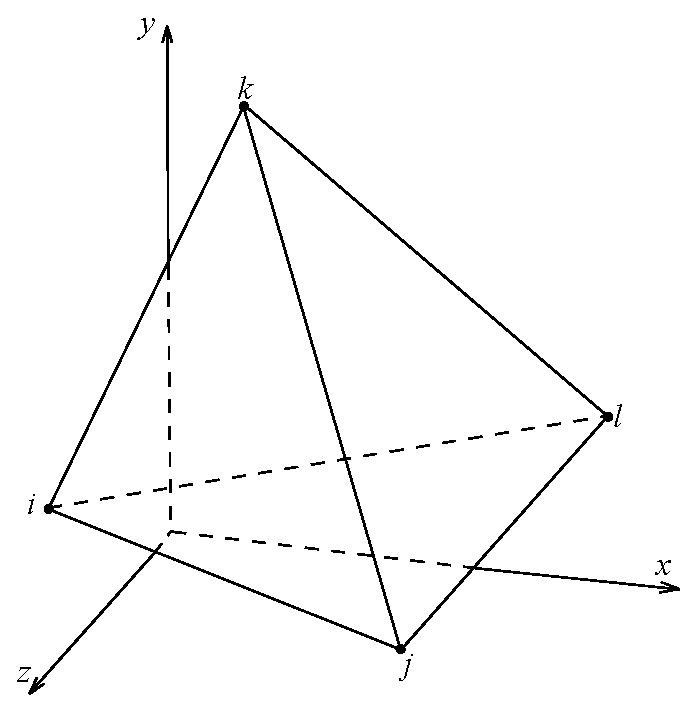
\includegraphics[angle=0,width=9cm]{tetraeder}\\[2mm]
%{\small Подрисуночный текст. Подрисуночный текст}
%\caption{Подпись к рисунку. Дополнительная информация}\label{lykov_am}
\caption{Нумерация узлов тетраэдра}\label{fig:tetraeder}
\end{center}
\end{figure}

Текст...

\newpage
\section*{Выводы}
\addcontentsline{toc}{section}{Выводы}

Выводы иногда удобно писать с новой страницы.
\chapter{ЕЩЁ ГЛАВА} \label{chapter:4}



\section[Ссылка на другой раздел или параграф]{Ссылка на другой раздел или параграф}



Как показано в разделе \ref{ch1-2}, самка черепахи не плывёт на север.


\section[Ссылка на свои статьи]{Ссылка на свои статьи}

Этот вопрос исследован в \cite{myarticle1}.

Этот вопрос исследован в \cite{myarticle2, myarticle3}.

Этот вопрос исследован в \cite{myarticle4, myarticle5}.

Этот вопрос исследован в \cite{myarticle6}.


%\clearpage 
\section*{Выводы}
\addcontentsline{toc}{section}{Выводы}

Текст...
\chapter{ЕЩЁ ГЛАВА} \label{chapter5}

\section[Пример альбомного листа]{Пример альбомного листа}



Бла-бла-бла... на рисунке \ref{img:point1-1}.



\begin{landscape}

\begin{figure}[hp]
\begin{center}
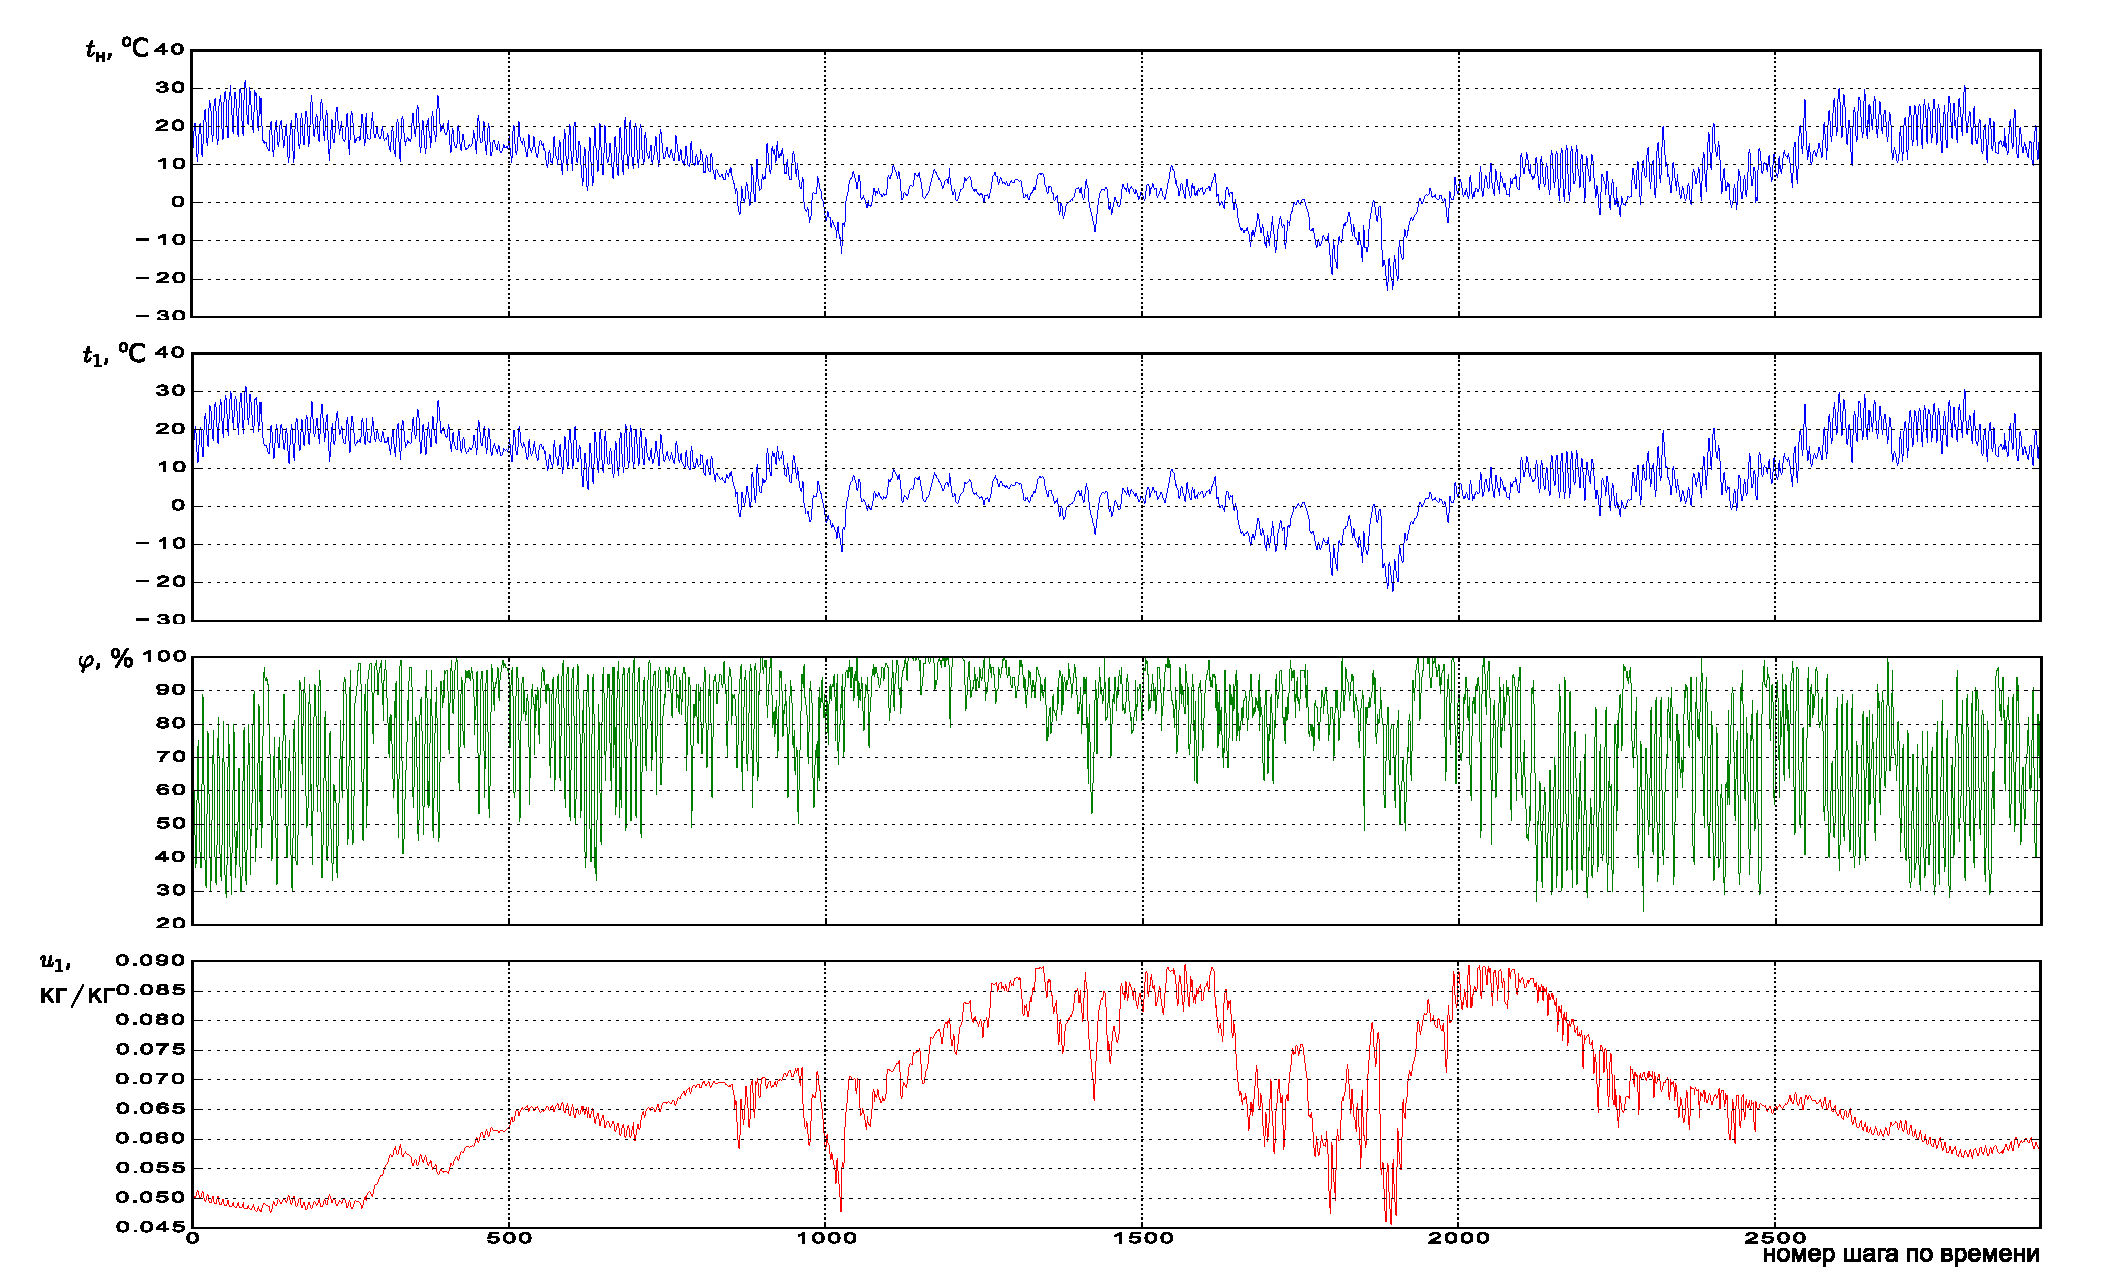
\includegraphics[angle=0,width=25cm]{ch5-point1-1}\\[2mm]
\caption {Рисунок сделан с помощью Matplotlib}\label{img:point1-1}
\end{center}
\end{figure}

\end{landscape}





%\newpage
\section*{Выводы}
\addcontentsline{toc}{section}{Выводы}

Текст...



%ЗАКЛЮЧЕНИЕ
%\chapter*{ЗАКЛЮЧЕНИЕ}
\addcontentsline{toc}{chapter}{ЗАКЛЮЧЕНИЕ}

\vspace{-10pt}
\subsection*{Основные научные результаты диссертации}

\vspace{-16pt}
%\subsubsection*{1.}
\textbf{1.~}
О-го-го!!!~\cite{myarticle1, myarticle2}.


\textbf{2.~}
Э-ге-гей!~\cite{myarticle3, myarticle4, myarticle5}.

Хе-хе-хе!!!~\cite{myarticle4, myarticle5}.


\textbf{3.~}
Э-э-эх!~\cite{myarticle6}.




\vspace{-10pt}
\ifthenelse{\value{isthesis}=1}{\newpage}{}
\subsection*{Рекомендации по практическому использованию результатов}

\vspace{-16pt}

У-у-ух!
\chapter*{ЗАКЛЮЧЕНИЕ}
\addcontentsline{toc}{chapter}{ЗАКЛЮЧЕНИЕ}

\vspace{-10pt}
\subsection*{Основные научные результаты диссертации}

\vspace{-16pt}
%\subsubsection*{1.}
\textbf{1.~}
О-го-го!!!~\cite{myarticle1, myarticle2}.


\textbf{2.~}
Э-ге-гей!~\cite{myarticle3, myarticle4, myarticle5}.

Хе-хе-хе!!!~\cite{myarticle4, myarticle5}.


\textbf{3.~}
Э-э-эх!~\cite{myarticle6}.




\vspace{-10pt}
\ifthenelse{\value{isthesis}=1}{\newpage}{}
\subsection*{Рекомендации по практическому использованию результатов}

\vspace{-16pt}

У-у-ух!


%БИБЛИОГРАФИЧЕСКИЙ СПИСОК
\chapter*{БИБЛИОГРАФИЧЕСКИЙ СПИСОК}
\addcontentsline{toc}{chapter}{БИБЛИОГРАФИЧЕСКИЙ СПИСОК}

%Библиография соискателя
%%\renewcommand{\mybibname}{}

\section*{Список публикаций соискателя}
\addcontentsline{toc}{section}{Список публикаций соискателя}%

\renewcommand{\mybibname}{\normalsize \mbox{Статьи} в \mbox{изданиях,} \mbox{включенных} в \mbox{перечни} \mbox{научных} \mbox{изданий} \mbox{для опубликования} \mbox{результатов} \mbox{диссертационных} \mbox{исследований}}

\begin{mybibliography}{10}
\def\selectlanguageifdefined#1{
\expandafter\ifx\csname date#1\endcsname\relax
\else\language\csname l@#1\endcsname\fi}
\ifx\undefined\url\def\url#1{{\small #1}}\else\fi
\ifx\undefined\BibUrl\def\BibUrl#1{\url{#1}}\else\fi
\ifx\undefined\BibAnnote\long\def\BibAnnote#1{}\else\fi
\ifx\undefined\BibEmph\def\BibEmph#1{\emph{#1}}\else\fi


% #1
\bibitem{myarticle1}
\selectlanguageifdefined{russian}
Название~статьи 1 / ~А.~А.~Автор1, ~А.~А.~Автор2, ~А.~А.~Автор3. ~А.~А.~Автор4~// ~Название~ ~Журнала. "---
\newblock 2006. "---
\newblock {\cyr\textnumero}~8. "---\newblock {\cyr\CYRS.}~5--9.


%#2
\bibitem{myarticle2}
\selectlanguageifdefined{russian}
Название~статьи 2 / ~А.~А.~Автор1, ~А.~А.~Автор2, ~А.~А.~Автор3, ~А.~А.~Автор4~// ~Название~ ~Журнала. "---
\newblock 2006. "---
\newblock {\cyr\textnumero}~8. "---\newblock {\cyr\CYRS.}~5--9.



\end{mybibliography}


\renewcommand{\mybibname}{\normalsize \mbox{Статьи в научно-технических журналах}}

\begin{mybibliography}{10}
\def\selectlanguageifdefined#1{
\expandafter\ifx\csname date#1\endcsname\relax
\else\language\csname l@#1\endcsname\fi}
\ifx\undefined\url\def\url#1{{\small #1}}\else\fi
\ifx\undefined\BibUrl\def\BibUrl#1{\url{#1}}\else\fi
\ifx\undefined\BibAnnote\long\def\BibAnnote#1{}\else\fi
\ifx\undefined\BibEmph\def\BibEmph#1{\emph{#1}}\else\fi

\setcounter{enumiv}{2} %тут вставить номер по порядку публикации из предыдущего раздела (здесь это номер 2  (см. выше %#2))

% #3
%эта НЕ ВАК
\bibitem{myarticle3}
\selectlanguageifdefined{russian}
Автор1,~А.~А. Влияние процессов ...~/ А.~А.~Автор1, А.~А.~Автор2~// 
  Журнал. "---
\newblock 2007. "---
\newblock {\cyr\textnumero} 7(40). "---
\newblock {\cyr\CYRS.}~58--61.

% #4
%эта НЕ ВАК
\bibitem{myarticle4}
\selectlanguageifdefined{russian}
Автор1,~А.~А. Влияние процессов ...~/ А.~А.~Автор1, А.~А.~Автор2, А.~А.~Автор3~// 
  Журнал. "---
\newblock 2013. "---
\newblock {\cyr\textnumero}~5. "---
\newblock {\cyr\CYRS.}~132--133.

\end{mybibliography}



\renewcommand{\mybibname}{\normalsize \mbox{Материалы} \mbox{докладов} на \mbox{конференциях,} \mbox{семинарах,} \mbox{тезисы} \mbox{докладов}}

\begin{mybibliography}{10}
\def\selectlanguageifdefined#1{
\expandafter\ifx\csname date#1\endcsname\relax
\else\language\csname l@#1\endcsname\fi}
\ifx\undefined\url\def\url#1{{\small #1}}\else\fi
\ifx\undefined\BibUrl\def\BibUrl#1{\url{#1}}\else\fi
\ifx\undefined\BibAnnote\long\def\BibAnnote#1{}\else\fi
\ifx\undefined\BibEmph\def\BibEmph#1{\emph{#1}}\else\fi

\setcounter{enumiv}{4} %тут вставить номер по порядку публикации из предыдущего раздела (здесь это номер 4)

%конференции

% #5
\bibitem{myarticle5}
\selectlanguageifdefined{russian}
Название ~/ А.~А.~Автор1, А.~А.~Автор2, А.~А.~Автор3,
  А.~А.~Автор4~// Наука -- образованию, производству, экономике: материалы
  Десятой междунар. науч.-техн. конф., Минск, 18–19 апр. 2006~г.: в~2~т.~/ Белорус. нац. техн. ун-т;
редкол.: И.~И.~Иванов, С.~С.~Сидоров, З.~З.~Забывайко. "---
\newblock \CYRT.~1. "---
\newblock Минск, 2006. "---
\newblock {\cyr\CYRS.}~11--19.

% #6
\bibitem{myarticle6}
\selectlanguageifdefined{russian}
Автор1,~А.~А. Название статьи~/ А.~А.~Автор1, А.~А.~Автор2~//
  Наука -- образованию, производству, экономике: материалы Пятой междунар. науч.-техн. конф., Минск, 11–12 апр. 2006~г.: в~12~т.~/ Белорус. нац. техн. ун-т;
редкол.: И.~И.~Иванов, С.~С.~Сидоров, З.~З.~Забывайко. "---
\newblock \CYRT.~1. "---
\newblock Минск, 2006. "---
\newblock {\cyr\CYRS.}~1--3.

\end{mybibliography}

%\renewcommand{\mybibname}{}

\section*{Список публикаций соискателя}
\addcontentsline{toc}{section}{Список публикаций соискателя}%

\renewcommand{\mybibname}{\normalsize \mbox{Статьи} в \mbox{изданиях,} \mbox{включенных} в \mbox{перечни} \mbox{научных} \mbox{изданий} \mbox{для опубликования} \mbox{результатов} \mbox{диссертационных} \mbox{исследований}}

\begin{mybibliography}{10}
\def\selectlanguageifdefined#1{
\expandafter\ifx\csname date#1\endcsname\relax
\else\language\csname l@#1\endcsname\fi}
\ifx\undefined\url\def\url#1{{\small #1}}\else\fi
\ifx\undefined\BibUrl\def\BibUrl#1{\url{#1}}\else\fi
\ifx\undefined\BibAnnote\long\def\BibAnnote#1{}\else\fi
\ifx\undefined\BibEmph\def\BibEmph#1{\emph{#1}}\else\fi


% #1
\bibitem{myarticle1}
\selectlanguageifdefined{russian}
Название~статьи 1 / ~А.~А.~Автор1, ~А.~А.~Автор2, ~А.~А.~Автор3. ~А.~А.~Автор4~// ~Название~ ~Журнала. "---
\newblock 2006. "---
\newblock {\cyr\textnumero}~8. "---\newblock {\cyr\CYRS.}~5--9.


%#2
\bibitem{myarticle2}
\selectlanguageifdefined{russian}
Название~статьи 2 / ~А.~А.~Автор1, ~А.~А.~Автор2, ~А.~А.~Автор3, ~А.~А.~Автор4~// ~Название~ ~Журнала. "---
\newblock 2006. "---
\newblock {\cyr\textnumero}~8. "---\newblock {\cyr\CYRS.}~5--9.



\end{mybibliography}


\renewcommand{\mybibname}{\normalsize \mbox{Статьи в научно-технических журналах}}

\begin{mybibliography}{10}
\def\selectlanguageifdefined#1{
\expandafter\ifx\csname date#1\endcsname\relax
\else\language\csname l@#1\endcsname\fi}
\ifx\undefined\url\def\url#1{{\small #1}}\else\fi
\ifx\undefined\BibUrl\def\BibUrl#1{\url{#1}}\else\fi
\ifx\undefined\BibAnnote\long\def\BibAnnote#1{}\else\fi
\ifx\undefined\BibEmph\def\BibEmph#1{\emph{#1}}\else\fi

\setcounter{enumiv}{2} %тут вставить номер по порядку публикации из предыдущего раздела (здесь это номер 2  (см. выше %#2))

% #3
%эта НЕ ВАК
\bibitem{myarticle3}
\selectlanguageifdefined{russian}
Автор1,~А.~А. Влияние процессов ...~/ А.~А.~Автор1, А.~А.~Автор2~// 
  Журнал. "---
\newblock 2007. "---
\newblock {\cyr\textnumero} 7(40). "---
\newblock {\cyr\CYRS.}~58--61.

% #4
%эта НЕ ВАК
\bibitem{myarticle4}
\selectlanguageifdefined{russian}
Автор1,~А.~А. Влияние процессов ...~/ А.~А.~Автор1, А.~А.~Автор2, А.~А.~Автор3~// 
  Журнал. "---
\newblock 2013. "---
\newblock {\cyr\textnumero}~5. "---
\newblock {\cyr\CYRS.}~132--133.

\end{mybibliography}



\renewcommand{\mybibname}{\normalsize \mbox{Материалы} \mbox{докладов} на \mbox{конференциях,} \mbox{семинарах,} \mbox{тезисы} \mbox{докладов}}

\begin{mybibliography}{10}
\def\selectlanguageifdefined#1{
\expandafter\ifx\csname date#1\endcsname\relax
\else\language\csname l@#1\endcsname\fi}
\ifx\undefined\url\def\url#1{{\small #1}}\else\fi
\ifx\undefined\BibUrl\def\BibUrl#1{\url{#1}}\else\fi
\ifx\undefined\BibAnnote\long\def\BibAnnote#1{}\else\fi
\ifx\undefined\BibEmph\def\BibEmph#1{\emph{#1}}\else\fi

\setcounter{enumiv}{4} %тут вставить номер по порядку публикации из предыдущего раздела (здесь это номер 4)

%конференции

% #5
\bibitem{myarticle5}
\selectlanguageifdefined{russian}
Название ~/ А.~А.~Автор1, А.~А.~Автор2, А.~А.~Автор3,
  А.~А.~Автор4~// Наука -- образованию, производству, экономике: материалы
  Десятой междунар. науч.-техн. конф., Минск, 18–19 апр. 2006~г.: в~2~т.~/ Белорус. нац. техн. ун-т;
редкол.: И.~И.~Иванов, С.~С.~Сидоров, З.~З.~Забывайко. "---
\newblock \CYRT.~1. "---
\newblock Минск, 2006. "---
\newblock {\cyr\CYRS.}~11--19.

% #6
\bibitem{myarticle6}
\selectlanguageifdefined{russian}
Автор1,~А.~А. Название статьи~/ А.~А.~Автор1, А.~А.~Автор2~//
  Наука -- образованию, производству, экономике: материалы Пятой междунар. науч.-техн. конф., Минск, 11–12 апр. 2006~г.: в~12~т.~/ Белорус. нац. техн. ун-т;
редкол.: И.~И.~Иванов, С.~С.~Сидоров, З.~З.~Забывайко. "---
\newblock \CYRT.~1. "---
\newblock Минск, 2006. "---
\newblock {\cyr\CYRS.}~1--3.

\end{mybibliography}


\bibliographystyle{gost71s2003}
\bibliography{bibliography}


%ПРИЛОЖЕНИЯ
\appendix
\chapter{Оформление приложений}
\label{app:1}

Оформление приложений начинается заданием команды \verb|\appendix|, которая изменяет стиль оформления документа. После данной команды, команда \verb|\chapter{Название}| задает не новые главы, а новые приложения, которые нумеруются буквами. Изменяется нумерация и у других элементов, таких как рисунки, таблицы и формулы, примеры которых приведены ниже (см. рисунок \ref{app:fig}, формулу (\ref{app:eq}) и таблицу \ref{app:tab}).

\begin{figure}[ht!]
\begin{center}
\includegraphics[angle=270,width=7cm]{test}\\
\caption{Подпись к рисунку. Дополнительная информация}
\label{app:fig}
\end{center}
\end{figure}

\begin{equation}\label{app:eq}
V = x^4 - 2 x^2,
\end{equation}
\begin{eqrem}
$x$ -- координата частицы.
\end{eqrem}

\begin{table}[h]
\caption{Характеристики процессов формирования волокон}
\begin{center}
\begin{tabular}{|>{\small}l|>{\small}c|>{\small}c|}
\hline
Наименование показателей & Вискоза & Камилон \\
\hline
Максимальная фильерная вытяжка, \% &12 &80\\
\hline
Температура осадительной ванны, \textcelsius &50 &20\\
\hline
Максимальная кратность вытягивания, \% &100 &30\\
\hline
\end{tabular}\label{app:tab}
\end{center}
\end{table}


\section{Раздел в приложении \ref{app:1}}

Приложение может разбиваться на разделы, подразделы и пункты с использованием стандартных команд секционирования.

\chapter{Сцепленные шаблоны диссертации, автореферата и презентации}\label{app:template}

Ниже представлена таблица \ref{table}, которая дает визуальное представление структуры сцепленных шаблонов диссертации, автореферата, презентации и списка вспомогательных файлов, которые включены в главные файлы через команду \verb|\include{имя файла}|.

Удобство использования сцепленных шаблонов заключаетсяв отсутсвии надобности дублировать одни и те же данные в разных документах. Например, положения выносимые на защиту должны дублироваться в диссертации, автореферате и презентации. Использование файла \textit{statements.tex}, которое содержит положения и используется во всех указанных выше документах, значительно упрощает работу над диссертацией и исключает необходимость постоянно следить за согласованностью положений в разных документах. То же касается частей диссертации, которые также должны быть и в автореферате (введение, общая характеристика работы, заключение и рекомендации по практическому использованию результатов).

\begin{table}[t]
\caption{Таблица, поясняющая структуру и связи в сцепленных шаблонах диссертации, автореферата и презентации}\label{table}
\begin{center}
\begin{tabular}{|p{58mm}|p{48mm}|p{49mm}|}
\hline
\large \bfseries ДИССЕРТАЦИЯ & \large \bfseries АВТОРЕФЕРАТ & \large \bfseries ПРЕЗЕНТАЦИЯ \\[2mm]
\hline
\multicolumn{3}{|c|}{\bfseries Главный файл}\\
\hline
\itshape THESIS.tex & \itshape ABSTRACT-PhD.tex & \itshape PRESENTATION.tex \\
\hline
\multicolumn{3}{|c|}{\bfseries Включенные файлы}\\
\hline
\multicolumn{3}{|c|}{\textit{statements.tex} -- положения, выносимые на защиту}\\
\hline
\multicolumn{3}{|p{16cm}|}{Рисунки хранятся в папке \textit{``fig''} в pdf формате. Обработка теховского файла производится pdfLaTeX. Для обычного LaTeXa нужны EPS рисунки.}\\
\hline
\textit{definitions.tex} -- список определений,
\newline \textit{titlepage.tex} -- титульная страница,
\newline \textit{thesisintro.tex} -- начало диссертации  &  \bfseries \large --- &
\textit{beamerthemeMinsk.sty} - стиль ``Минск'' для презентации (можно использовать любой другой стиль, см. \cite{beamer}) \\
\hline
\multicolumn{2}{|c|}{\textit{intro.tex} -- введение} & \bfseries \large --- \\
\hline
\multicolumn{2}{|c|}{\textit{characteristics.tex} -- общая характеристика работы} & \bfseries \large --- \\
\hline
\textit{chapter1.tex, chapter2.tex, chapter3.tex, chapter4.tex} -- четыре главы & \bfseries \large ---   & \bfseries \large --- \\
\hline
\multicolumn{2}{|c|}{\textit{conclusions.tex} -- заключение} & \bfseries \large --- \\
\hline
\multicolumn{2}{|p{11cm}|}{\textit{recommendations.tex} -- рекомендации по практическому использованию результатов} & \bfseries \large --- \\
\hline
\textit{bib.tex} -- библиографический список + статьи автора & \bfseries \large ---   & \bfseries \large --- \\
\hline
\multicolumn{2}{|p{11cm}|}{\textit{bibmypapers.tex} -- статьи соискателя в научных журналах} & \bfseries \large ---  \\
\hline
\multicolumn{2}{|p{11cm}|}{\textit{bibmyreports.tex} -- статьи соискателя в материалах конференций} & \bfseries \large ---  \\
\hline
\textit{appendix.tex} -- приложения.  & \bfseries \large ---   & \bfseries \large --- \\
\hline
\end{tabular}
\end{center}

\end{table}


\chapter{Нумерация приложений}

Согласно требованиям, приложения следует обозначать заглавными буквами русского алфавита. В данном классе это организуется автоматически при задании команды начала нового приложения \verb|\chapter{Название приложения}|. Но нужно обратить внимание на то, что не все буквы могут быть использованы для нумерации. Буквы Ё, З, Й, О, Ч, Ь, Ы, Ъ должны быть исключены из нумерации. В классе использована функция \verb|\Asbuk| для формы представления счетчика приложений, которая сама не включает в нумерацию буквы Ё, Й, Ь, Ы, Ъ. Но буквы З, О, Ч, остаются. Для их исключения перед приложением, которое может получить неподходящую букву, нужно изменить счетчик приложений {\itshape chapter}, используя команду \verb|\addtocounter{chapter}{1}|.

Для нумерации приложений также можно пользоваться буквами латинского алфавита. Для этого сразу после команды  \verb|\appendix|, задающей начало приложений, нужно переопределить форму командой: \verb|\renewcommand{\thechapter}{\Alph{chapter}}|. Исключение лишних букв I и O из нумерации осуществляется описанным выше способом.


\chapter{Таблица с больш\'{и}м количеством строк}
\label{app:table}

Ниже приведен пример таблицы с большим количеством строк. Основные объяснения по оформлению данного типа таблиц приведены в подразделе~\ref{sec:ltable} и книге \cite[раздел 12.5]{Kotelnikov}.

\begin{longtable}{|l|c|c|}
\caption{Подпись к таблице с большим количеством строк. Таблица занимает две страницы.}
\label{tab:long}
 \\ \hline
Боковик & Первый столбец & Второй столбец \\ \hline
        \endfirsthead
\multicolumn{3}{l}{Продолжение таблицы \ref{tab:long}}
\\ \hline
Боковик & Первый столбец & Второй столбец \\ \hline
        \endhead
        \endfoot
    \hline  \endlastfoot

Название & Элемент первого столбца & Элемент второго столбца \\
Название & Элемент первого столбца & Элемент второго столбца \\
Название & Элемент первого столбца & Элемент второго столбца \\
Название & Элемент первого столбца & Элемент второго столбца \\
Название & Элемент первого столбца & Элемент второго столбца \\
Название & Элемент первого столбца & Элемент второго столбца \\
Название & Элемент первого столбца & Элемент второго столбца \\
Название & Элемент первого столбца & Элемент второго столбца \\
Название & Элемент первого столбца & Элемент второго столбца \\
Название & Элемент первого столбца & Элемент второго столбца \\
Название & Элемент первого столбца & Элемент второго столбца \\
Название & Элемент первого столбца & Элемент второго столбца \\
Название & Элемент первого столбца & Элемент второго столбца \\
Название & Элемент первого столбца & Элемент второго столбца \\
Название & Элемент первого столбца & Элемент второго столбца \\
Название & Элемент первого столбца & Элемент второго столбца \\
Название & Элемент первого столбца & Элемент второго столбца \\
Название & Элемент первого столбца & Элемент второго столбца \\
Название & Элемент первого столбца & Элемент второго столбца \\
Название & Элемент первого столбца & Элемент второго столбца \\
Название & Элемент первого столбца & Элемент второго столбца \\
Название & Элемент первого столбца & Элемент второго столбца \\
Название & Элемент первого столбца & Элемент второго столбца \\
Название & Элемент первого столбца & Элемент второго столбца \\
Название & Элемент первого столбца & Элемент второго столбца \\
Название & Элемент первого столбца & Элемент второго столбца \\
Название & Элемент первого столбца & Элемент второго столбца \\
Название & Элемент первого столбца & Элемент второго столбца \\
Название & Элемент первого столбца & Элемент второго столбца \\
Название & Элемент первого столбца & Элемент второго столбца \\
Название & Элемент первого столбца & Элемент второго столбца \\
Название & Элемент первого столбца & Элемент второго столбца \\
Название & Элемент первого столбца & Элемент второго столбца \\
Название & Элемент первого столбца & Элемент второго столбца \\
Название & Элемент первого столбца & Элемент второго столбца \\
Название & Элемент первого столбца & Элемент второго столбца \\
Название & Элемент первого столбца & Элемент второго столбца \\
Название & Элемент первого столбца & Элемент второго столбца \\
Название & Элемент первого столбца & Элемент второго столбца \\
Название & Элемент первого столбца & Элемент второго столбца \\
Название & Элемент первого столбца & Элемент второго столбца \\
Название & Элемент первого столбца & Элемент второго столбца \\
\end{longtable}
%\end{table}

\chapter{Таблица с больш\'{и}м количеством столбцов}
\label{app:gtable}

Ниже приведен пример таблицы с большим количеством столбцов. Основные объяснения по оформлению данного типа таблиц приведены в подразделе~\ref{sec:gtable}.

\begin{table}[h]
\caption{Характеристики процессов формирования волокон из гидратцеллюлозы}
\label{tab:g}
\begin{tabular}{|>{\small}l|>{\small}c|>{\small}c|>{\small}c|}
\hline
Наименование показателей & Вискоза & Камилон & Волокно \textnumero 3 \\
\hline
Максимальная фильерная вытяжка, \% &12 &80 &42 \\
\hline
Температура осадительной ванны, \textcelsius &20 &12 &80 \\
\hline
Максимальная кратность вытягивания, \% &100 &32 &84 \\
\hline
\end{tabular}

\smallskip
Продолжение таблицы \ref{tab:g}\\
\begin{tabular}{|>{\small}l|>{\small}c|>{\small}c|>{\small}c|}
\hline
Наименование показателей & Волокно \textnumero 4 & Волокно \textnumero 5 & Волокно \textnumero 6 \\
\hline
Максимальная фильерная вытяжка, \% &80 &42 &83 \\
\hline
Температура осадительной ванны, \textcelsius &20 &12 &80 \\
\hline
Максимальная кратность вытягивания, \% &100 &32 &84 \\
\hline
\end{tabular}

\smallskip
Окончание таблицы \ref{tab:g}\\
\begin{tabular}{|>{\small}l|>{\small}c|>{\small}c|>{\small}c|}
\hline
Наименование показателей & Волокно \textnumero 7 & Волокно \textnumero 8 & Волокно \textnumero 9 \\
\hline
Максимальная фильерная вытяжка, \% &80 &42 &82 \\
\hline
Температура осадительной ванны, \textcelsius &40 &12 &80 \\
\hline
Максимальная кратность вытягивания, \% &100 &34 &84 \\
\hline
\end{tabular}


\end{table}





\end{document}


